\documentclass[tikz, border = 5pt]{standalone}

\begin{document}
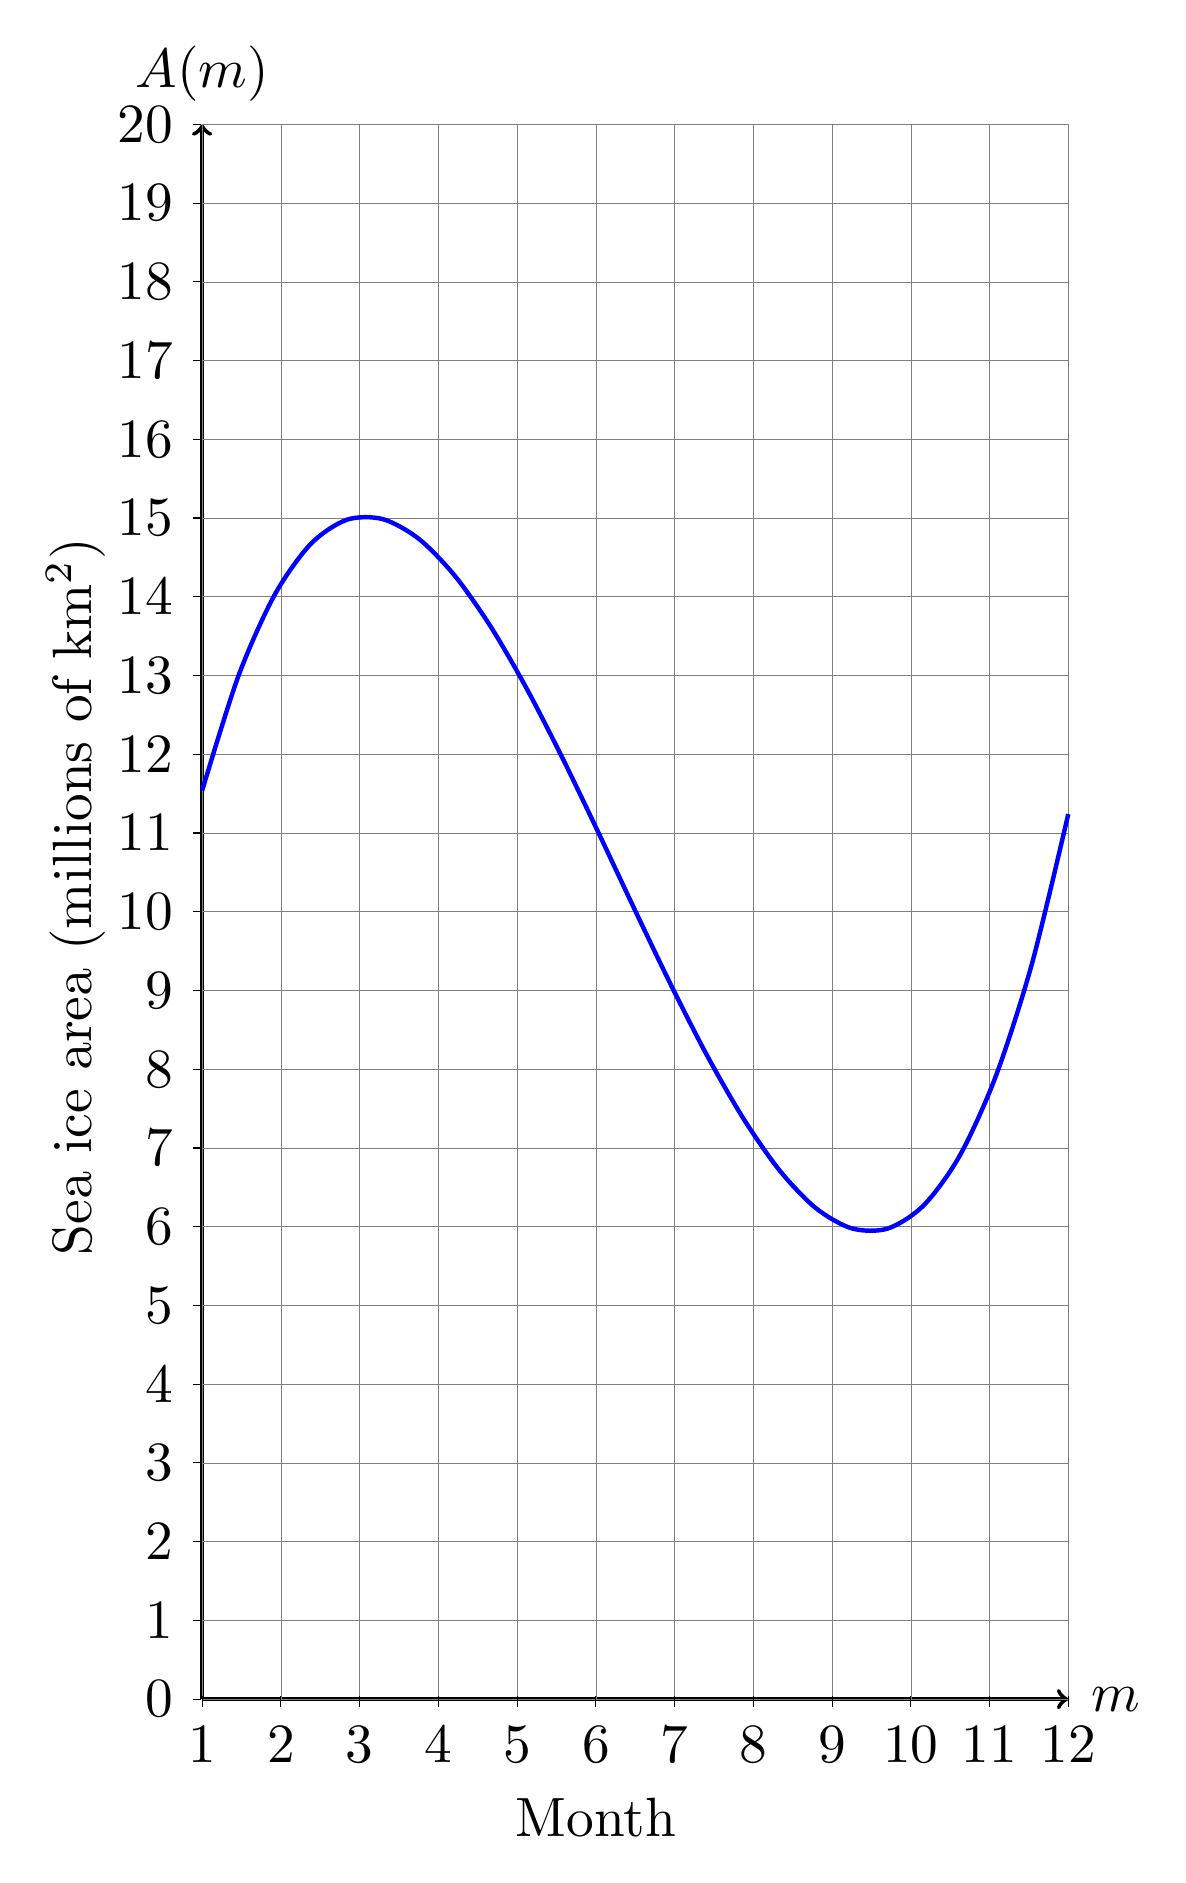
\begin{tikzpicture}
% axis
\draw[ultra thick, ->] (1, 0) -- (1, 20) node[above, black, scale=2] {$A(m)$};
\draw[ultra thick, ->] (1, 0) -- (12, 0) node[right, black, scale=2] {$m$};
\node[rotate=90, scale=2] at (-0.8,10,-0.5) {Sea ice area (millions of km$^2$)};
\node[scale=2] at (6,-1.5) {Month};

% grid
\draw[help lines, step = 1cm] (1, 0) grid (12, 20);

%ticks
\foreach \x in {1,...,12}
  \draw (\x,1pt) -- (\x,-3pt) node[anchor=north, scale=2] {\x};
\foreach \y in {0,...,20}
  \draw (28pt,\y) -- (25pt,\y) node[anchor=east, scale=2] {\y};

% graph
\draw[ultra thick, scale=1, domain=1:12,smooth,variable=\x, blue] plot ({\x},{  0.069*\x*\x*\x - 1.3*\x*\x + 6.04*\x + 6.73});

\end{tikzpicture}
\end{document}
